%basic concept
\section{基本概念}
\begin{enumerate}
\item 路径\label{ll:lj}
路径是曲线(也被称为贝兹曲线)。路径在GIMP中是很容易学习和使用的。路径工具是非常强大的,它允许你设计复杂的东西。要使用GIMP的路径工具,你必须首先创建一个路径,然后对路径进行描边(指定特定风格的路径--颜色,宽度,图案等)。

\item 颜色四种模式\label{ll:ms}
\begin{description}
\item[SHB] 人眼对颜色的感知模式。分别对应饱和度(趋向白色)[Saturation]、色相(纯度)[Hue]、明度(趋向黑色)[Brightness]。当R=G=B时,颜色无色相。
\item[RGB] 光线对颜色的感知模式。分别对应红色、绿色和蓝色。对于8bit的像素点来说,[255,255,255]代表白,[0,0,0]代表黑。颜色混合如下图\ref{ll:ms:rgb}
\begin{figure}[!htbp]
	\centering
	\caption{RGB颜色混合} 
    	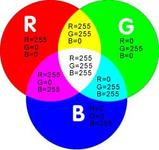
\includegraphics[scale=0.65]{figs/concept_RGB.jpg}
    	\label{ll:ms:rgb}
\end{figure}
\item[CMYK] 油墨对颜色的感知模式。分别对应青色、品红色、黄色和黑色。理想情况下,[100,100,100]代表黑,[0,0,0]代表白。因为无法提取出100\%纯度的CMY三种颜料,所以混合后无法形成纯黑。所以用单独的黑色颜料来代替三者的混合。即现实打印中代表黑的是[0,0,0,100],代表白的是[0,0,0,0]。其他的则是[x,x,x,0]。注意上图\ref{ll:ms:rgb}中,RGB两两混合后即为CMY。
\item[LAB] 大自然对颜色的感知模式。$LAB>CMYK,LAB>RGB$。
\end{description}
\end{enumerate}





\clearpage